\subsubsection{Immagini}
Alcune immagini medio-grandi risultano cliccabili ma la maggior 
parte delle immagini grandi riguardanti i prodotti non risultano cliccabili.
\begin{figure}[ht]
\centering
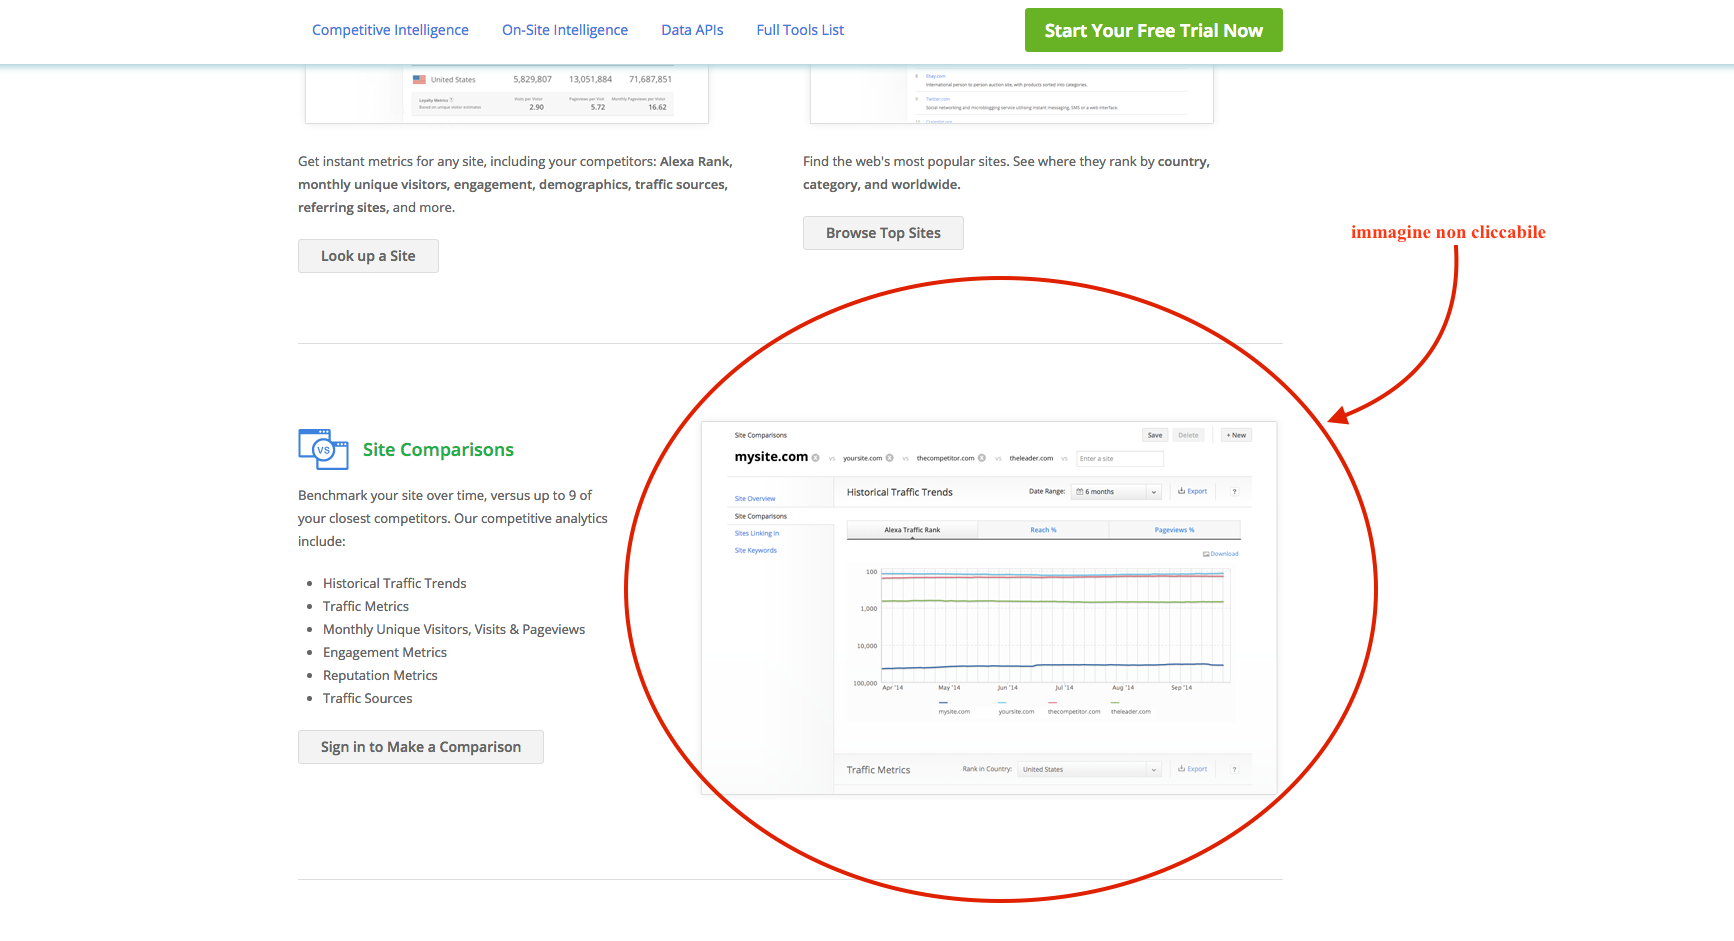
\includegraphics[scale=0.22,keepaspectratio]{{figure/4/images0}.png}
\caption{Esempio di immagine non cliccabile}
\end{figure}
\FloatBarrier 
La motivazione è data dall'utilizzo della metafora link/pulsante (vedi 
\ref{sezioni}) che esclude l'uso di immagini come link. Questa scelta risulta
controintuitiva poichè il 20\% degli utenti quando vede un'immagine la clicca
aspettandosi di essere redirezionato alla pagina correlata.\\
Risultato : \textit{5.5}